
%%%%%%%%%%%%%%%%%%%%%%%%%%%%%%%%%%%%%%%%%%%%%%%%%%%%%%%%%%%%%%%%%%%%%
%% This is a (brief) model paper using the achemso class
%% The document class accepts keyval options, which should include
%% the target journal and optionally the manuscript type.
%%%%%%%%%%%%%%%%%%%%%%%%%%%%%%%%%%%%%%%%%%%%%%%%%%%%%%%%%%%%%%%%%%%%%
\documentclass[journal=jacsat,manuscript=article]{achemso}

%%%%%%%%%%%%%%%%%%%%%%%%%%%%%%%%%%%%%%%%%%%%%%%%%%%%%%%%%%%%%%%%%%%%%
%% Place any additional packages needed here.  Only include packages
%% which are essential, to avoid problems later. Do NOT use any
%% packages which require e-TeX (for example etoolbox): the e-TeX
%% extensions are not currently available on the ACS conversion
%% servers.
%%%%%%%%%%%%%%%%%%%%%%%%%%%%%%%%%%%%%%%%%%%%%%%%%%%%%%%%%%%%%%%%%%%%%
\usepackage[version=3]{mhchem} % Formula subscripts using \ce{}
\usepackage[colorlinks,linkcolor=red]{hyperref}

%%%%%%%%%%%%%%%%%%%%%%%%%%%%%%%%%%%%%%%%%%%%%%%%%%%%%%%%%%%%%%%%%%%%%
%% If issues arise when submitting your manuscript, you may want to
%% un-comment the next line.  This provides information on the
%% version of every file you have used.
%%%%%%%%%%%%%%%%%%%%%%%%%%%%%%%%%%%%%%%%%%%%%%%%%%%%%%%%%%%%%%%%%%%%%
%%\listfiles

%%%%%%%%%%%%%%%%%%%%%%%%%%%%%%%%%%%%%%%%%%%%%%%%%%%%%%%%%%%%%%%%%%%%%
%% Place any additional macros here.  Please use \newcommand* where
%% possible, and avoid layout-changing macros (which are not used
%% when typesetting).
%%%%%%%%%%%%%%%%%%%%%%%%%%%%%%%%%%%%%%%%%%%%%%%%%%%%%%%%%%%%%%%%%%%%%
\newcommand*\mycommand[1]{\texttt{\emph{#1}}}

%%%%%%%%%%%%%%%%%%%%%%%%%%%%%%%%%%%%%%%%%%%%%%%%%%%%%%%%%%%%%%%%%%%%%
%% Meta-data block
%% ---------------
%% Each author should be given as a separate \author command.
%%
%% Corresponding authors should have an e-mail given after the author
%% name as an \email command. Phone and fax numbers can be given
%% using \phone and \fax, respectively; this information is optional.
%%
%% The affiliation of authors is given after the authors; each
%% \affiliation command applies to all preceding authors not already
%% assigned an affiliation.
%%
%% The affiliation takes an option argument for the short name.  This
%% will typically be something like "University of Somewhere".
%%
%% The \altaffiliation macro should be used for new address, etc.
%% On the other hand, \alsoaffiliation is used on a per author basis
%% when authors are associated with multiple institutions.
%%%%%%%%%%%%%%%%%%%%%%%%%%%%%%%%%%%%%%%%%%%%%%%%%%%%%%%%%%%%%%%%%%%%%
\author{SX1916115 Jingtang Zhang}
\email{jingtangzhang@nuaa.edu.cn}
\affiliation[NUAA]
{CCST, NUAA, Nanjing, China}

%%%%%%%%%%%%%%%%%%%%%%%%%%%%%%%%%%%%%%%%%%%%%%%%%%%%%%%%%%%%%%%%%%%%%
%% The document title should be given as usual. Some journals require
%% a running title from the author: this should be supplied as an
%% optional argument to \title.
%%%%%%%%%%%%%%%%%%%%%%%%%%%%%%%%%%%%%%%%%%%%%%%%%%%%%%%%%%%%%%%%%%%%%
\title[An \textsf{achemso} demo]
  {Machine Learning Project Report}

%%%%%%%%%%%%%%%%%%%%%%%%%%%%%%%%%%%%%%%%%%%%%%%%%%%%%%%%%%%%%%%%%%%%%
%% Some journals require a list of abbreviations or keywords to be
%% supplied. These should be set up here, and will be printed after
%% the title and author information, if needed.
%%%%%%%%%%%%%%%%%%%%%%%%%%%%%%%%%%%%%%%%%%%%%%%%%%%%%%%%%%%%%%%%%%%%%
% \abbreviations{IR,NMR,UV}
% \keywords{American Chemical Society, \LaTeX}

\begin{document}
%%%%%%%%%%%%%%%%%%%%%%%%%%%%%%%%%%%%%%%%%%%%%%%%%%%%%%%%%%%%%%%%%%%%%
%% The manuscript does not need to include \maketitle, which is
%% executed automatically.  The document should begin with an
%% abstract, if appropriate.  If one is given and should not be, the
%% contents will be gobbled.
%%%%%%%%%%%%%%%%%%%%%%%%%%%%%%%%%%%%%%%%%%%%%%%%%%%%%%%%%%%%%%%%%%%%%
% \begin{abstract}
%   This is an example document for the \textsf{achemso} document
%   class, intended for submissions to the American Chemical Society
%   for publication. The class is based on the standard \LaTeXe\
%   \textsf{report} file, and does not seek to reproduce the appearance
%   of a published paper.

%   This is an abstract for the \textsf{achemso} document class
%   demonstration document.  An abstract is only allowed for certain
%   manuscript types.  The selection of \texttt{journal} and
%   \texttt{manuscript} will determine if an abstract is valid.  If
%   not, the class will issue an appropriate error.
% \end{abstract}

%%%%%%%%%%%%%%%%%%%%%%%%%%%%%%%%%%%%%%%%%%%%%%%%%%%%%%%%%%%%%%%%%%%%%
%% Start the main part of the manuscript here.
%%%%%%%%%%%%%%%%%%%%%%%%%%%%%%%%%%%%%%%%%%%%%%%%%%%%%%%%%%%%%%%%%%%%%
\section{About the Task}

Our task is to finish a competition on \emph{kaggle}, which is a platform
for machine learning competitions. Specifically, our task is based on a
famous computer game called \emph{PLAYERUNKNOWN’S BATTLEGROUNDS (PUBG)}.
In this game, up to 100 players will be dropped onto an island called Erangel
empty-handed. They must explore, scavenge, and eliminate other players until
only one of them is left standing, all while the play zone continues to
shrink.

We are given some anomymized player data from 65000 games. The data is split
into training set and testing set. In the training set, we have the data describing
the player's performance, like various kinds of killing count, or the
moving distance on a car or under water. And also, we have a winning placement
percentage \textbf{winPlacePerc}, ranging from 0 to 1, where 1 corresponds to
1st place, and 0 corresponds to last place. This percentage is the target of
the prediction. In the testing set, we have all of the columns in the training
set, except the \textbf{winPlacePer} column. Our task is to predict this column
as precise as possible. The final score is calculated by the mean absolute error
between the prediction and the groud-truth.

\section{Analysis and Motivation}

\subsection{Version 1}

For the given training data, we can see that it either describe the behavior of a player
or the metadata of a match. According to my experience of playing computer games when I
was a teenager, the final score of a match is strongly related to the match type.
For different match types, there are different rules and strategies, which may affect the
players' data like walking distance and killing count. So my first motivation is to
split the training set by different match types.

And also, during different matches, one player tend to perform differently. He may shoot
well in one game, while missing everything he shoot in another game. My second motivation
is to train a model for each single game.

From the course \emph{Machine Learning}, I have learned about the power of ensemble learning.
So I tried to use all models of the same match type to predict a record from the corresponding
match type, and get the average value as the final prediction result.

\subsection{Version 2}

In the algorithm of version 1, the data for training a model comes from a single game,
containing less than 100 rows, which is too few for training a model empirically.
So I tried to use more data for each model's training process. However, the amount of
data for each match type is totally different. As a result, it is impossible to train models
for match types without much data.

My solution is to train models by different types of match. I split the whole training
set into 100 parts, and use each part to train a model. Each part contains about 45000 rows
of data from different match types. While predicting a record, I 
use all of the 100 models to predict and use the average value as the final result.

\section{Algorithm and Implementation}

\subsection{Version 1}

For the first version of my algorithm, I choose the following features: ["walkDistance",
"killStreaks", "rideDistance", "kills", "heals", "boosts", "damageDealt", "weaponsAcquired",
"headshotKills", "teamKills", "roadKills", "swimDistance", "revives", "assists", "killPlace",
"longestKill", "vehicleDestroys"]. The reason is that, these features are all used to describe a 
player, instead of a match. In my opinion, since I train a model for each single match,
the features describing the match are meaningless, because they are the same for the same match.

I choose \textbf{Decision Tree regressor} as the algorithm. The reason is that it can 
save the effort of decomposition, since I don't know which feature is more important for 
the result. It can judge the best feature for me automatically.

In order to train a model from a match, I sorted the whole training data by match type and matchID.
For each matchID, I trained a model using all rows with this matchID, and added the model to the 
set of corresponding match type. During prediction, I used all the models of that match type 
to calculate the average prediction value, which is an application of ensemble learning: considering
the matches are inherently independent to each other, the model generated from each match 
can do prediction independently.

Specifically, to speed up the prediction, for match types with much more data, which corresponds
to more models, I randomly sampled part of the models for prediction by a max predictor threshold.
Also, I implemented the program in a multi-processes way, 
which can fully utilize the multi-core CPU. The source code is available at my
\href{https://github.com/mrdrivingduck/pugb-finish-placement-prediction/blob/master/src/main_multi_process_version.py}{GitHub}.

\subsection{Version 2}

For the second version of my algorithm, I trained 100 models with about 45000 rows of data each,
and used all models together to predict a record. I tried several ensumble learning algorithms,
including \textbf{XGBoost regressor}, \textbf{Random Forest regressor}, \textbf{AdaBoost regressor}
and \textbf{Gradient Boosting regressor}. They are all using ensemble method inside.
I integrated them together for the second time of ensemble learning.
The source code is available at my
\href{https://github.com/mrdrivingduck/pugb-finish-placement-prediction/blob/master/src/main_ensemble.py}{GitHub}.

\section{Results and Evaluation}

\subsection{Version 1}

For the version 1 algorithm, I tried different parameters of max predictor threshold.
If a match type contains more models than the threshold, then only models of the
threshold would get involved into the prediction.

At first, I introduced this parameter for speeding up the prection process. However,
according to the experiment, I found a greater threshold would not get a better score.
I used the threshold of 500, 1000, 1500, 2000, among which 1500 gets the following best score,
while 1000 is not better than 500 and 2000 is not better than 1500.

\begin{figure}
  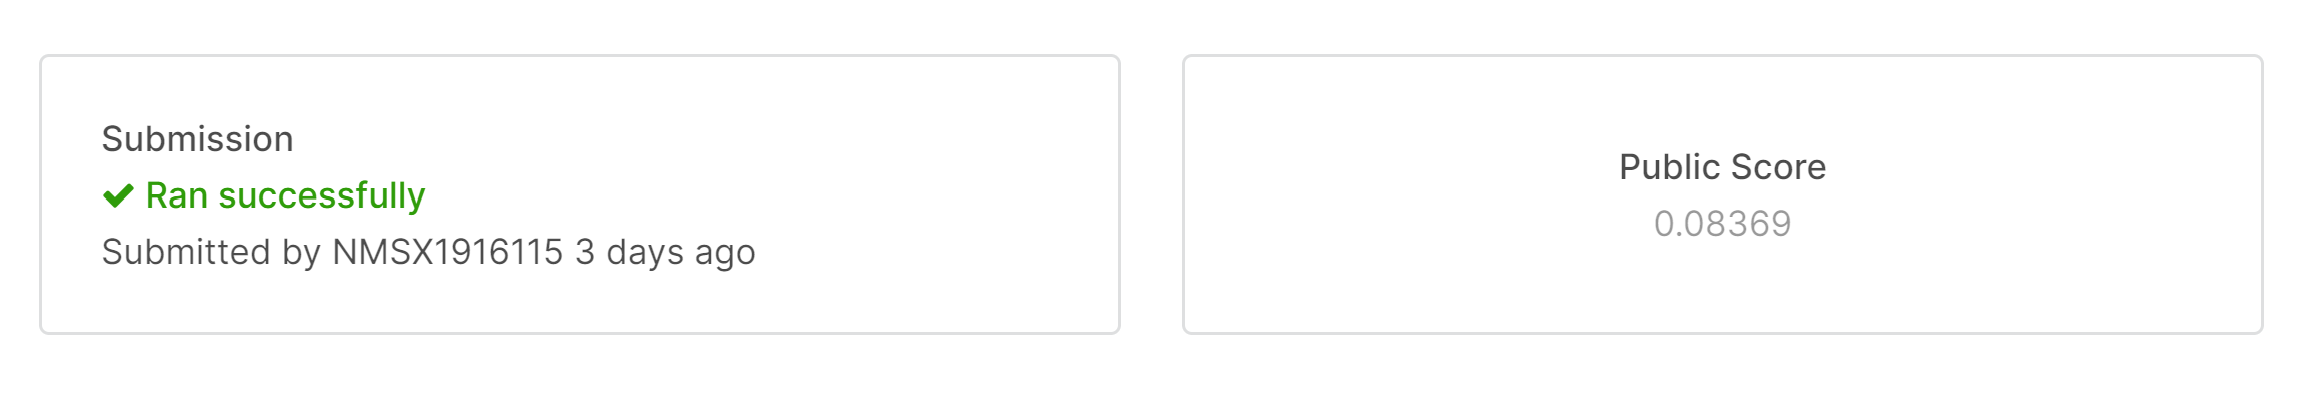
\includegraphics[height=2.4cm]{img/res-version-1.png}
\end{figure}

\subsection{Version 2}

For the version 2 algorithm, I just tried different ensemble learning method:
\textbf{XGBoost regressor}, \textbf{Random Forest regressor}, \textbf{AdaBoost regressor}
and \textbf{Gradient Boosting regressor}, among which Random Forest regressor 
got the following best score.

\begin{figure}
  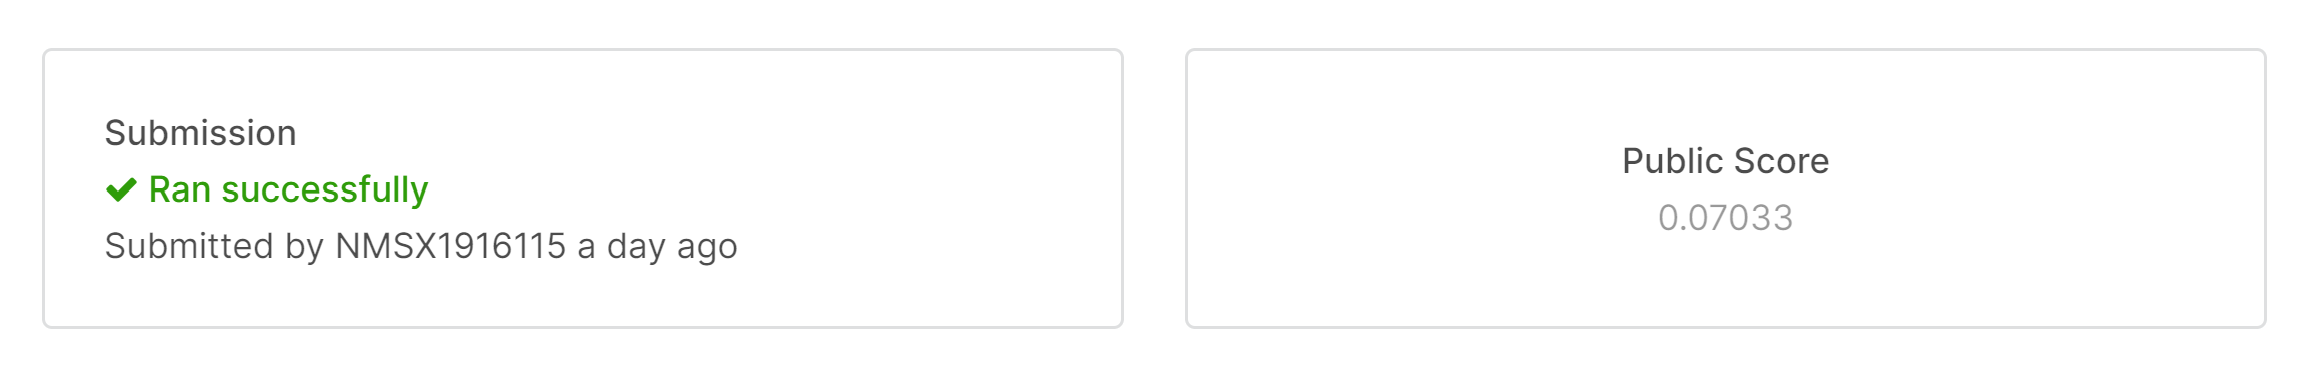
\includegraphics[height=2.4cm]{img/res-version-2.png}
\end{figure}


\section{Thoughts}

I didn't do much work about the features in my experiment,
which should be an important part in machine learning.
In fact, I tried to use \emph{Principal Components Analysis} to cut off some features, 
but it didn't work well. I referred to some high score solutions after my experiment,
and found that their feature engineering was much more complex.
Some of them even generated some features from the given training data,
and got a very good result.
I guess the better feature engineering is why they can get a higher score.

\end{document}
